\documentclass[border=10pt]{standalone}
\usepackage{tikz}
\usetikzlibrary{3d}

\begin{document}
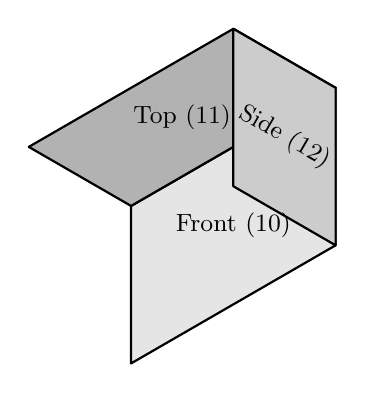
\begin{tikzpicture}[
  x  = {(0.866cm, 0.5cm)},
  y  = {(0cm, 1cm)},
  z  = {(-0.866cm, 0.5cm)},
  line join=round
]
  \def\W{3} \def\H{2} \def\D{1.5}

  % 앞면
  \fill[white!90!black, draw=black, thick]
    (0,0,0) -- (\W,0,0) -- (\W,\H,0) -- (0,\H,0) -- cycle;
  % 윗면
  \fill[white!70!black, draw=black, thick]
    (0,\H,0) -- (\W,\H,0) -- (\W,\H,\D) -- (0,\H,\D) -- cycle;
  % 옆면
  \fill[white!80!black, draw=black, thick]
    (\W,0,0) -- (\W,0,\D) -- (\W,\H,\D) -- (\W,\H,0) -- cycle;

  % 참조번호
  \node at (1.5,1,0)     [font=\small] {Front (10)};
  \node at (1.5,\H,0.75) [font=\small] {Top (11)};
  \node at (\W,1,0.75)   [font=\small, rotate=-30] {Side (12)};
\end{tikzpicture}
\end{document}
